\let\negmedspace\undefined
\let\negthickspace\undefined
\documentclass[journal]{IEEEtran}
\usepackage[a5paper, margin=10mm, onecolumn]{geometry}
\usepackage{tfrupee} 

\setlength{\headheight}{1cm}
\setlength{\headsep}{0mm}     

\usepackage{gvv-book}
\usepackage{gvv}
\usepackage{cite}
\usepackage{amsmath,amssymb,amsfonts,amsthm}
\usepackage{algorithmic}
\usepackage{graphicx}
\usepackage{textcomp}
\usepackage{xcolor}
\usepackage{txfonts}
\usepackage{listings}
\usepackage{enumitem}
\usepackage{mathtools}
\usepackage{gensymb}
\usepackage{comment}
\usepackage[breaklinks=true]{hyperref}
\usepackage{tkz-euclide} 
\usepackage{listings}
\def\inputGnumericTable{}                                 
\usepackage[latin1]{inputenc}                                
\usepackage{color}                                            
\usepackage{array}                                            
\usepackage{longtable}                                       
\usepackage{calc}                                             
\usepackage{multirow}                                         
\usepackage{hhline}                                           
\usepackage{ifthen}                                           
\usepackage{lscape}
\usepackage{circuitikz}


\tikzstyle{block} = [rectangle, draw, fill=blue!20, 
    text width=4em, text centered, rounded corners, minimum height=3em]
\tikzstyle{sum} = [draw, fill=blue!10, circle, minimum size=1cm, node distance=1.5cm]
\tikzstyle{input} = [coordinate]
\tikzstyle{output} = [coordinate]

\begin{document}

\bibliographystyle{IEEEtran}
\vspace{3cm}

\title{4.11.21}
\author{EE25BTECH11044 - Sai Hasini Pappula}
 \maketitle
{\let\newpage\relax\maketitle}

\renewcommand{\thefigure}{\theenumi}
\renewcommand{\thetable}{\theenumi}
\setlength{\intextsep}{10pt} 

\numberwithin{equation}{enumi}
\numberwithin{figure}{enumi}
\renewcommand{\thetable}{\theenumi}
\section*{Question}
Find the equation of the plane passing through the line of intersection of the planes
\begin{equation}
    r.(2\hat{i} + 2\hat{j} - 3\hat{k} )= 7
\end{equation}
\begin{equation}
    r.(2\hat{i} + 5\hat{j}+ 3\hat{k} )= 9
\end{equation}

such that the intercepts made by the plane on the $x$-axis and $z$-axis are equal.

\section*{Solution}

\subsection*{Step 1: Represent as a system}

The general plane through the intersection of the planes can be written as:
\begin{equation}
(2 + 2\lambda)x + (2 + 5\lambda)y + (-3 + 3\lambda)z = 7 + 9\lambda, \
\end{equation}

where \(\lambda\) is a scalar.  

We can represent the plane coefficients as a **row vector**:
\[
\begin{bmatrix} a & b & c \end{bmatrix} = \begin{bmatrix} 2 + 2\lambda & 2 + 5\lambda & -3 + 3\lambda \end{bmatrix}, \quad
d = 7 + 9\lambda.
\]

---

\subsection*{Step 2: Express intercept condition as a matrix equation}

Let the plane intercepts on $x$ and $z$ axes be equal. \\ 

The $x$-intercept occurs when$y=0, z=0$ and the $z$-intercept occurs when $x=0, y=0$.  

This gives the system
\begin{equation}
\begin{bmatrix}
2 + 2\lambda & 0 & 0 \\
0 & 0 & -3 + 3\lambda
\end{bmatrix}
\begin{bmatrix} x_0 \\ y_0 \\ z_0 \end{bmatrix} =
\begin{bmatrix} 7 + 9\lambda \\ 7 + 9\lambda \end{bmatrix}. \label{eq:intercept_matrix}
\end{equation}

 we can write:
\begin{equation}
(2 + 2\lambda)x_0 = 7 + 9\lambda, \quad (-3 + 3\lambda) z_0 = 7 + 9\lambda. 
\end{equation}

Equal intercepts condition:
\begin{equation}
x_0 = z_0 \quad \Rightarrow \quad 2 + 2\lambda = -3 + 3\lambda \quad \Rightarrow \quad \lambda = 5. 
\end{equation}

---

\subsection*{Step 3: Form the plane equation matrix}

Substitute \(\lambda = 5\)

\[
\begin{bmatrix} a & b & c \end{bmatrix} = \begin{bmatrix} 2 + 10 & 2 + 25 & -3 + 15 \end{bmatrix} = \begin{bmatrix} 12 & 27 & 12 \end{bmatrix}, \quad d = 7 + 45 = 52.
\]

Hence, the plane equation is
\begin{equation}
12x + 27y + 12z = 52. 
\end{equation}
\begin{center}
    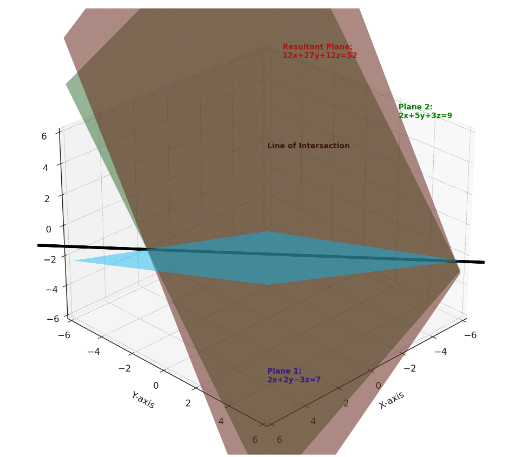
\includegraphics[width=0.8\columnwidth]{figs/plot8.png}
\end{center}
\end{document}